\documentclass[unicode,11pt,a4paper,oneside,numbers=endperiod,openany]{scrartcl}

\usepackage{ifthen}
\usepackage[utf8]{inputenc}
\usepackage{graphics}
\usepackage{graphicx}
\usepackage{hyperref}

\pagestyle{plain}
\voffset -5mm
\oddsidemargin  0mm
\evensidemargin -11mm
\marginparwidth 2cm
\marginparsep 0pt
\topmargin 0mm
\headheight 0pt
\headsep 0pt
\topskip 0pt        
\textheight 255mm
\textwidth 165mm

\newcommand{\duedate} {}
\newcommand{\setduedate}[1]{%
\renewcommand\duedate {Due date:~ #1}}
\newcommand\isassignment {false}
\newcommand{\setassignment}{\renewcommand\isassignment {true}}
\newcommand{\ifassignment}[1]{\ifthenelse{\boolean{\isassignment}}{#1}{}}
\newcommand{\ifnotassignment}[1]{\ifthenelse{\boolean{\isassignment}}{}{#1}}

\newcommand{\assignmentpolicy}{
\begin{table}[h]
\begin{center}
\scalebox{0.8} {%
\begin{tabular}{|p{0.02cm}p{16cm}|}
\hline
&\\
\multicolumn{2}{|c|}{\Large\textbf{HPC Lab 2020 ---  Submission Instructions}}\\
\multicolumn{2}{|c|}{\large\textbf{(Please, notice that following instructions are mandatory: }}\\
\multicolumn{2}{|c|}{\large\textbf{submissions that don't comply with, won't be considered)}}\\
&\\
\textbullet & Assignments must be submitted to \href{https://www.icorsi.ch/course/view.php?id=10049}{Icorsi} (i.e. in electronic format).\\
\textbullet & Provide both executable package and sources (e.g. C/C++ files, Matlab). 
If you are using libraries, please add them in the file. Sources must be organized in directories called:\\
\multicolumn{2}{|c|}{\textit{Project\_number\_lastname\_firstname}}\\
& and  the  file must be called:\\
\multicolumn{2}{|c|}{\textit{project\_number\_lastname\_firstname.zip}}\\
\multicolumn{2}{|c|}{\textit{project\_number\_lastname\_firstname.pdf}}\\
\textbullet &  The TAs will grade your project by reviewing your project write-up, and looking at the implementation 
                 you attempted, and benchmarking your code's performance.\\

\textbullet & You are allowed to discuss all questions with anyone you like; however: (i) your submission must list anyone you discussed problems with and (ii) you must write up your submission independently.\\
\hline
\end{tabular}
}
\end{center}
\end{table}
}
\newcommand{\punkte}[1]{\hspace{1ex}\emph{\mdseries\hfill(#1~\ifcase#1{Points}\or{Points}\else{Points}\fi)}}


\newcommand\serieheader[6]{
\thispagestyle{empty}%
\begin{flushleft}

\includegraphics[width=0.4\textwidth]{images/usi_inf.pdf}
\end{flushleft}
  \noindent%
  {\large\ignorespaces{\textbf{#1}}\hspace{\fill}\ignorespaces{ \textbf{#2}}}\\ \\%
  {\large\ignorespaces #3 \hspace{\fill}\ignorespaces #4}\\
  \noindent%
  \bigskip
  \hrule\par\bigskip\noindent%
  \bigskip {\ignorespaces {\Large{\textbf{#5}}}
  \hspace{\fill}\ignorespaces \large \ifthenelse{\boolean{\isassignment}}{\duedate}{#6}}
  \hrule\par\bigskip\noindent%  \linebreak
 }

\makeatletter
\def\enumerateMod{\ifnum \@enumdepth >3 \@toodeep\else
      \advance\@enumdepth \@ne
      \edef\@enumctr{enum\romannumeral\the\@enumdepth}\list
      {\csname label\@enumctr\endcsname}{\usecounter
        {\@enumctr}%%%? the following differs from "enumerate"
	\topsep0pt%
	\partopsep0pt%
	\itemsep0pt%
	\def\makelabel##1{\hss\llap{##1}}}\fi}
\let\endenumerateMod =\endlist
\makeatother




\usepackage{textcomp}





\begin{document}


\setassignment
\setduedate{30.10.2020 (midnight)}

\serieheader{High-Performance Computing Lab}{2020}{Student: Gabriele Berra}{Discussed with: -}{Solution for Project 4}{}
\newline

\assignmentpolicy



In this fourth assignment I have to complete a code in order to solve the Fisher's equation and, after that, parallelize it using openMP. The Fisher equation,
\begin{equation*}
	\frac{\partial s}{\partial t} = D \left(\frac{\partial^2 s}{\partial x^2} + \frac{\partial^2 s}{\partial y^2} \right) + Rs(1-s)
\end{equation*}
was first proposed by Ronald Fisher in 1937 in order to describe the dynamics of advantageous genes.\\
In our specific case we discretise its domain using a uniform grid in which we approximate the points with a second order finite difference approximation of the type:
\begin{equation*}
	\left(\frac{\partial^2 s}{\partial x^2} + \frac{\partial^2 s}{\partial y^2} \right)_{i,j} \approx \frac{1}{\Delta x^2} (-4s_{i,j}+s_{i-1,j}+s_{i+1,j}+s_{i,j-1}+s_{i,j+1})
\end{equation*}
And, for the time derivative: 
\begin{equation*}
	\left(\frac{\partial s}{\partial t}  \right)^k_{i,j} \approx \frac{1}{\Delta t}(s^k_{i,j} - s^{k-1}_{i,j})
\end{equation*}
In order to obtain an approximation we can reformulate the two equations above as follows: 
\begin{equation}\label{eq:s}
	f^k_{i,j} := [-(4+\alpha)s_{i,j}+s_{i-1,j}+ s_{i+1,j}+s_{i,j-1}+ s_{i,j+1}+ \beta s_{i,j}(1- s_{i,j})]^k + \alpha s^{k-1}_{i,j} = 0 
\end{equation}.
Since each equation is quadratic in $s$ we have to solve it using Newton's method for the roots of a function. The Newton's method is based on iteratively search the root of a function taking in considerations the derivatives and an initial guess $x_0$. Since we have $n^2$ derivatives for a given $k$, with the aim of calculating the inverse Jacobian matrix, we use a Conjugate Gradient solver to solve the linear system of equation given by rearranging the terms of the Newton's method:
\begin{equation*}
	[\mathbf{J}_{\mathbf{f}}(\mathbf{y}^l)]\delta \mathbf{y}^{l+1} = \mathbf{f}(\mathbf{y}^l)
\end{equation*}





\section{Task: Implementing the linear algebra functions and the stencil operators [40 Points]}
For this first task of the assignment 4 I have, on one hand, to implement the functions in the \textit{linalg.cpp} file and, on the other, to implement the missing stencil in the \textit{operators.cpp} file. I started tackling the implementation of the linear algebra functions by following the instructions given in the code. The script I implemented is the following:\\
\lstinputlisting[frame=single, breaklines=true, tabsize=3, firstline=46 ,lastline=139, language=C++]{project4_code/linalg.cpp}

In the \textit{operators.cpp} file I have to implement: the nested for loop for the interior grid points, the west boundary, inner north boundary and, inner south boundary. To do so I firstly have to understand the difference between the positions of the points in the grid and how to better calculate their approximation. We know from the theory that a generic inner point in the grid can be easily calculated with equation \ref{eq:s}. For the boundaries, I have to modify equation \ref{eq:s} since, on these points, some neighbours are missing (e.g. on the south-east corner the "south" and the "east" point are missing). The modified equations are the following:\\ \\For the west boundary:
  \lstinputlisting[frame=single, breaklines=true, tabsize=3, firstline=63 ,lastline=70, language=C++]{project4_code/operators.cpp}  
For the inner north boundary:
\lstinputlisting[frame=single, breaklines=true, tabsize=3, firstline=87 ,lastline=94, language=C++]{project4_code/operators.cpp} 
For the inner south boundary:
\lstinputlisting[frame=single, breaklines=true, tabsize=3, firstline=119 ,lastline=125, language=C++]{project4_code/operators.cpp}

\begin{figure}[h!]
\centering
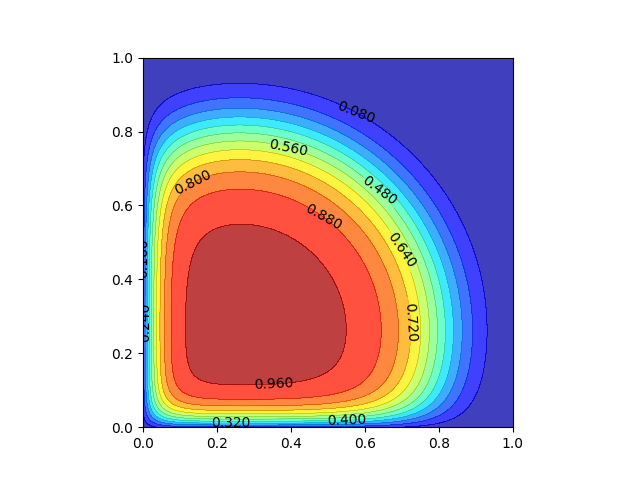
\includegraphics[width=\textwidth]{Figures/serialFig.png}
\caption{Serial plot with 128 x 128 grid points}\label{fig:serialPlot}
\end{figure}

 

\section{Task:  Adding OpenMP to the nonlinear PDE mini-app [60 Points]}
This second part of the assignment is divided into 5 subsections mainly focused on the parallelization of the code of the first part. These subsections are:
\begin{enumerate}
	\item Replace welcome message in main.cpp.
	\item Linear algebra kernel.
	\item The diffusion stencil.
	\item Strong scaling.
	\item Weak scaling.
\end{enumerate}

For the first point, the main issue - in my opinion - is how to "connect" the environment variable \textit{export OMP\_NUM\_THREADS=x} with a local variable in the \textit{main.cpp} script. I decided to solve this problem by adding the command \textit{omp\_get\_max\_threads()}, which gives as output the maximum number of threads that can be used in the parallel regions. I implemented it in the script as follows:\\
\lstinputlisting[frame=single, breaklines=true, tabsize=3, showstringspaces=false, firstline=103 ,lastline=114, language=C++]{project4_code/main.cpp}

For the second point I have to implement parallel section only in the linear algebra script. Since all the functions that I added have a \textit{for loop} inside, I decided to use the \textit{\# pragma omp parallel for} command in all of the functions. By doing so, I noticed that in \textit{hpc\_dot()} and \textit{hpc\_norm2()} adding only a \textit{parallel for} section is not enough to perform the correct calculations. Thus, since the variable \textit{result} is just a sum over the iterations of the previous loop, I used a \textit{reduction} clause to perform the parallelization. The code is reported below.
\lstinputlisting[frame=single, breaklines=true, tabsize=3, showstringspaces=false, firstline=46 ,lastline=149, language=C++]{project4_code/linalg_omp.cpp} 

After the parallelization of the \textit{linalg\_omp.cpp} script, I expect an increase in the performance since most of the operations are performed using linear algebra functions.
Comparing the results of this first step of parallelization - using 8 threads - with the serial version we can notice an improvement, in terms of performance - i.e. speed - both for the 128 x 128 grid and the 256 x 256 one. The results are reported in Table \ref{tab:linalgSP} (time expressed in seconds):

\begin{table}[h!]
\begin{center}
	\begin{tabular}{|c|c|c|}
		\hline
		\textbf{Grid Size} & \textbf{Serial Time} & \textbf{Parallel Time}\\
		\hline\hline
		128 x 128 & 1.22729 & 0.760295  \\
		\hline
		256 x 256  & 9.01825 & 3.72461  \\
		\hline
	\end{tabular}
\end{center}
\caption{Time with the serial version of \textit{linalg.cpp} and the parallel one using 8 threads}\label{tab:linalgSP}
\end{table}

The next step is to parallelize the \textit{operations\_omp.cpp} script. The parallelization of this script is non-trivial since we have to understand which of the for loops has to be parallel and which one does not. In my opinion, we have to think about how many iterations each loop has to do in order to achieve the correct result. If we consider a 10 x 10 grid, the inner point for which the script has to do the calculations are 64 while, in contrast, the boundary points are "only" 38. If we take in consideration a bigger grid, for example a 128 x 128, the points on the boundary are 508 and the inner points are 15'876. So for a bigger grid the nested loop - i.e. the loop that performs the operation in the inner point - has a major impact on the general performance and, thus, I focused my attention on the parallelization of the latter one.
The parallelized section of the code is reported below.\\
\lstinputlisting[frame=single, breaklines=true, tabsize=3, showstringspaces=false, firstline=39 ,lastline=49, language=C++]{project4_code/operators_omp.cpp} 

\subsection{Strong scaling}
As we know from the theory the \textit{strong scaling} is defined as the scalability of a specific threaded algorithm when the number of threads used increases and the problem size remains constant. In our case I tested the algorithm for different sizes and, for each, I tested the strong scalability. The results are summarized in the following Table \ref{tab:strongScaling} and Fig. \ref{fig:strongScaling} .


\begin{table}[h!]
\begin{center}
	\begin{tabular}{|c|c|c|c|c|c|}
		\hline
		\textbf{\# threads/Grid Size} & 64 x 64 & 128 x 128 & 256 x 256 & 512 x 512 & 1024 x 1024\\
		\hline
		1&0.196281&1.28041&8.81197&65.0061&717.519\\
		\hline
		2&0.187238&0.953788&6.15223&45.2533&408.307\\
		\hline
		3&0.162066&0.835927&5.02967&36.4704&345.568\\
		\hline
		4&0.165711&0.77066&4.43689&30.5576&346.456\\
		\hline
		5&0.175701&0.756458&4.1095&28.737&357.694\\
		\hline
		6&0.171196&0.752386&3.9769&26.9436&320.769\\
		\hline
		7&0.184268&0.768854&3.78487&26.2863&298.011\\
		\hline
		8&0.192468&0.773505&3.86266&24.5194&303.903\\
		\hline
		9&0.199429&0.763555&3.70059&25.2214&288.606\\
		\hline
		10&0.268303&0.776758&3.61467&23.8828&301.479\\
		\hline
	\end{tabular}
\end{center}
\caption{Strong scaling}\label{tab:strongScaling}
\end{table}

\begin{figure}[h!]
\centering
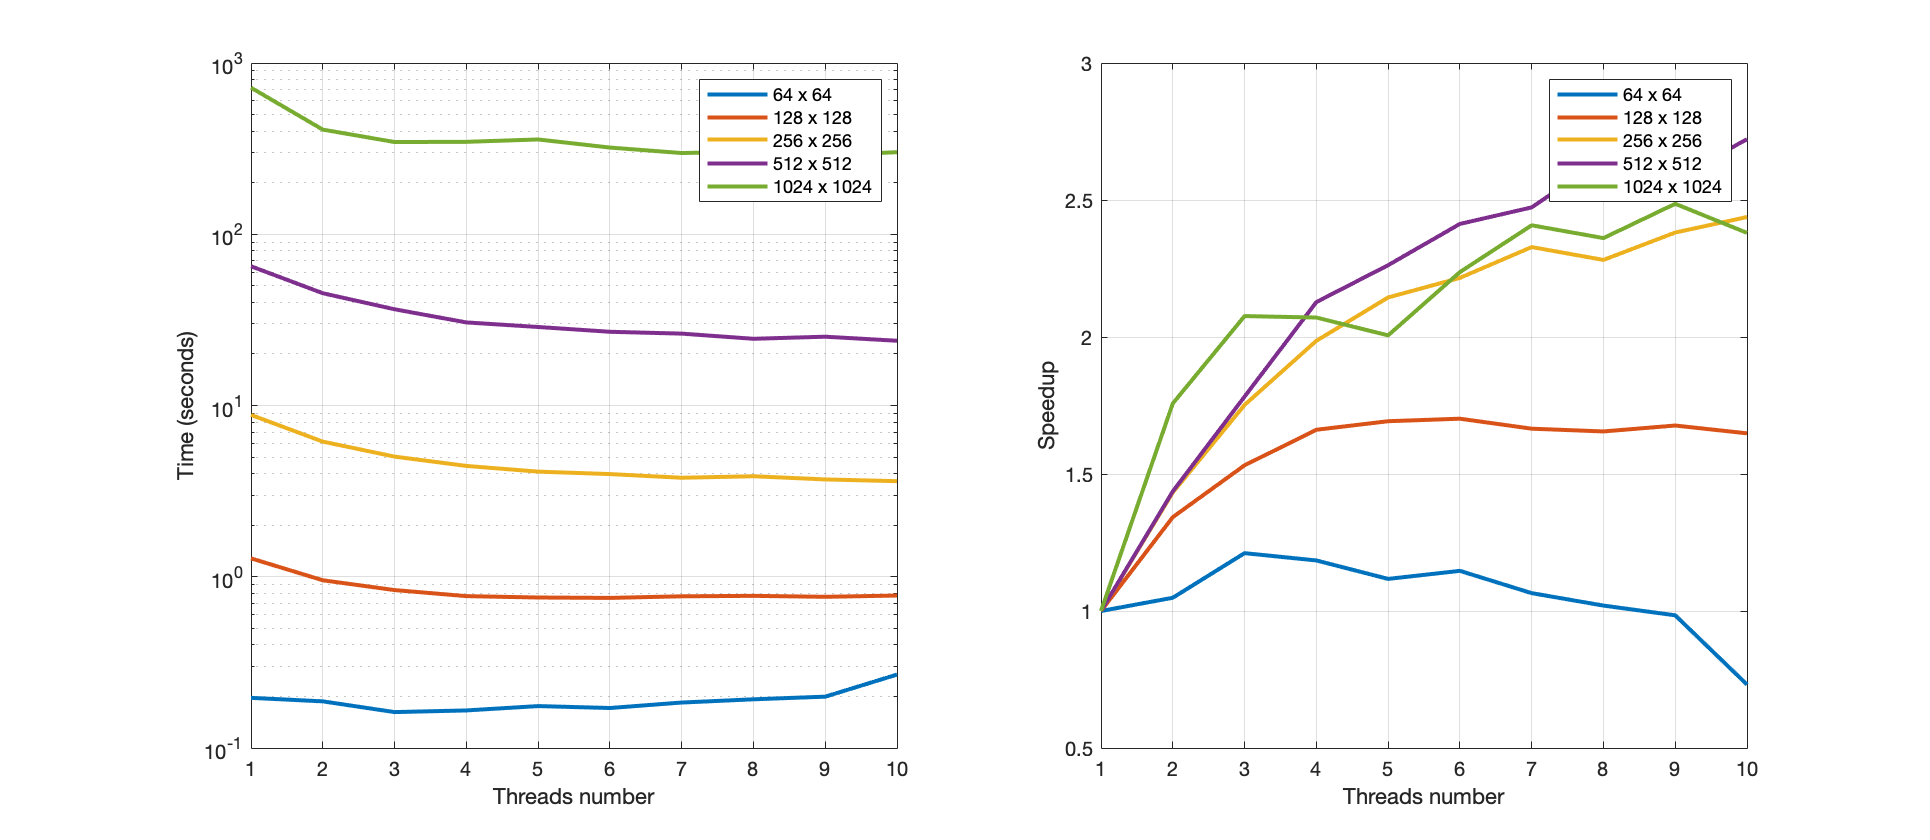
\includegraphics[width=\textwidth]{Figures/strongScaling.png}
\caption{Strong scaling and speedup}\label{fig:strongScaling}
\end{figure}

In general, as we can see in Fig. \ref{fig:strongScaling}, for any given size the code scales except for the 64 x 64 grid in which, an increase from 9 to 10 threads produces a worst performance compared to the one using only one thread. This is probably because the time for dividing the tasks between the threads in the parallel section and the computation time is greater than the computation time with one thread. In all the other cases is beneficial the usage of more threads, in particular for big grid sizes.    


\subsection{Weak scaling}
For this last section I will tackle the analysis of the weak scalability, which can be defined as follows: how the solution time varies with the number of processors for a fixed problem size per processor.\footnote{Source: https://en.wikipedia.org/wiki/Scalability\#Weak\_versus\_strong\_scaling} In my analysis I decided to use 1, 4 and 16 threads with problem sizes associated to each thread given by:
\begin{itemize}
	\item 64 x 64 for each thread, with the total problem size going from 64 x 64 (1 thread) to 128 x 128 (4 threads) and 256 x 256 (16 threads)
	\item  128 x 128 for each thread, with the total problem size going from 128 x 128 (1 thread) to 256 x 256 (4 threads) and 512 x 512 (16 threads)
	\item 256 x 256 for each thread, with the total problem size going from 256 x 256 (1 thread) to 512 x 512 (4 threads) and 1024 x 1024 (16 threads)
\end{itemize}


\begin{figure}[h!]
\centering
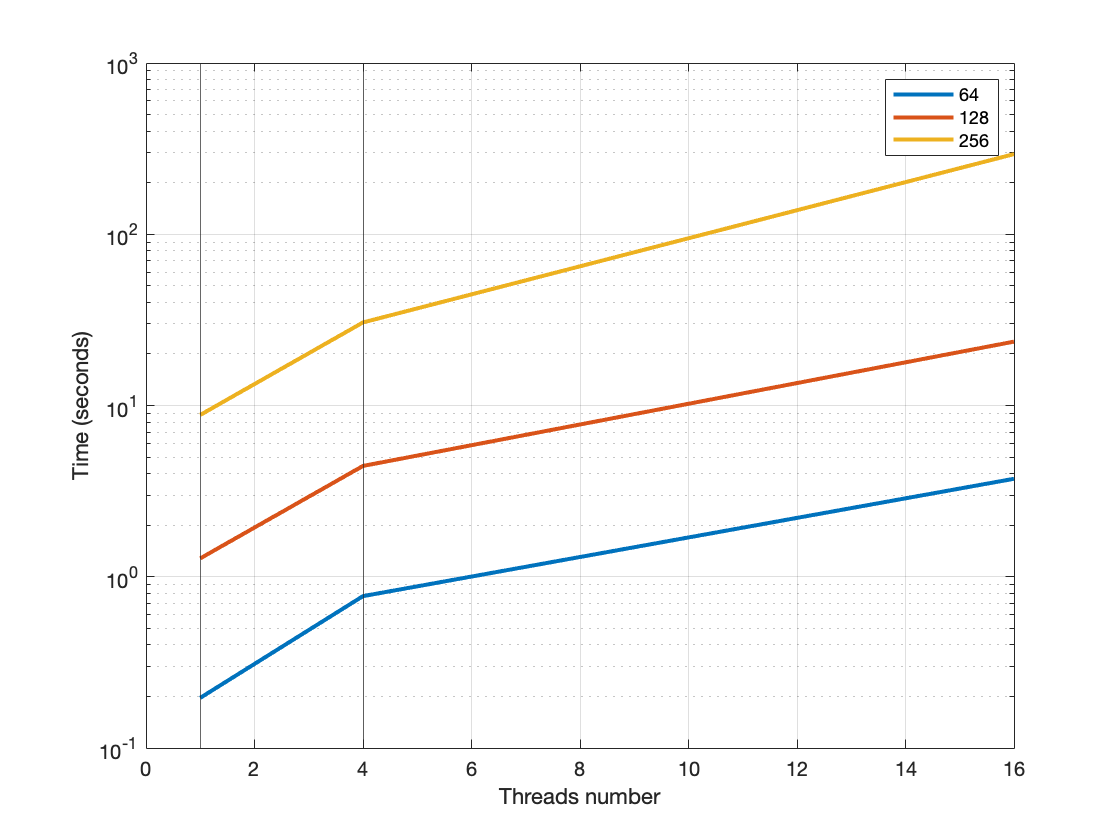
\includegraphics[width=\textwidth]{Figures/weakScaling.png}
\caption{Weak scaling with different initial size}\label{fig:weakScaling}
\end{figure}
As we can notice in Fig.\ref{fig:weakScaling} the time for the computation slightly increases due to the overhead of the threads since, for a constant problem size assigned to each thread, the time for the distribution of the tasks inside the parallel region increases, this cause the plot to be non-constant. 
















 



\end{document}
